\chapter{Introduction: Plasmas and Tokamak Plasmas}
    Nuclear fusion energy has the potential to provide a nearly unlimited source of clean and safe energy. Fusion reactions do not produce harmful greenhouse gases or long-lived radioactive waste and provide no risk of meltdown, and consequently offer a sustainable solution for meeting the world's growing demand for energy from a stable and renewable source: hydrogen (and its isotopes). With the world's energy demands continuously growing, fusion energy presents an attractive option for meeting these demands.

    \shortline
      
    Magnetic confinement reactors---devices that use strong magnetic fields to contain and control plasmas at exceedingly high temperatures in order to achieve fusion---have proven to be an effective leading option for producing and sustaining fusion over recent decades. Unlike other types of magnetic confinement reactors such as stellarators or Z-pinch devices, tokamaks have a relatively simple and well-studied design with comparatively straightforward engineering, making them easier to scale up to commercial-scale reactors. Under construction in southern France \cite{Claessens_2019}, the International Thermonuclear Experimental Reactor (ITER) will be the world's largest tokamak \cite{Meade_2009, ITER_plan}, building towards DEMO: a proposed class of demonstration tokamak, with a target for commercial operation in the 2050s.

    Because of these factors, tokamaks have received extensive funding and support from governments and private organizations around the world, making them potentially the most widely researched and developed fusion technology.

    These factors combined make tokamaks one of the world's best solutions for fusion energy, and arguably the most likely to achieve practical and commercial fusion in the coming decades.

    \begin{figure}[!ht]
        \centering
        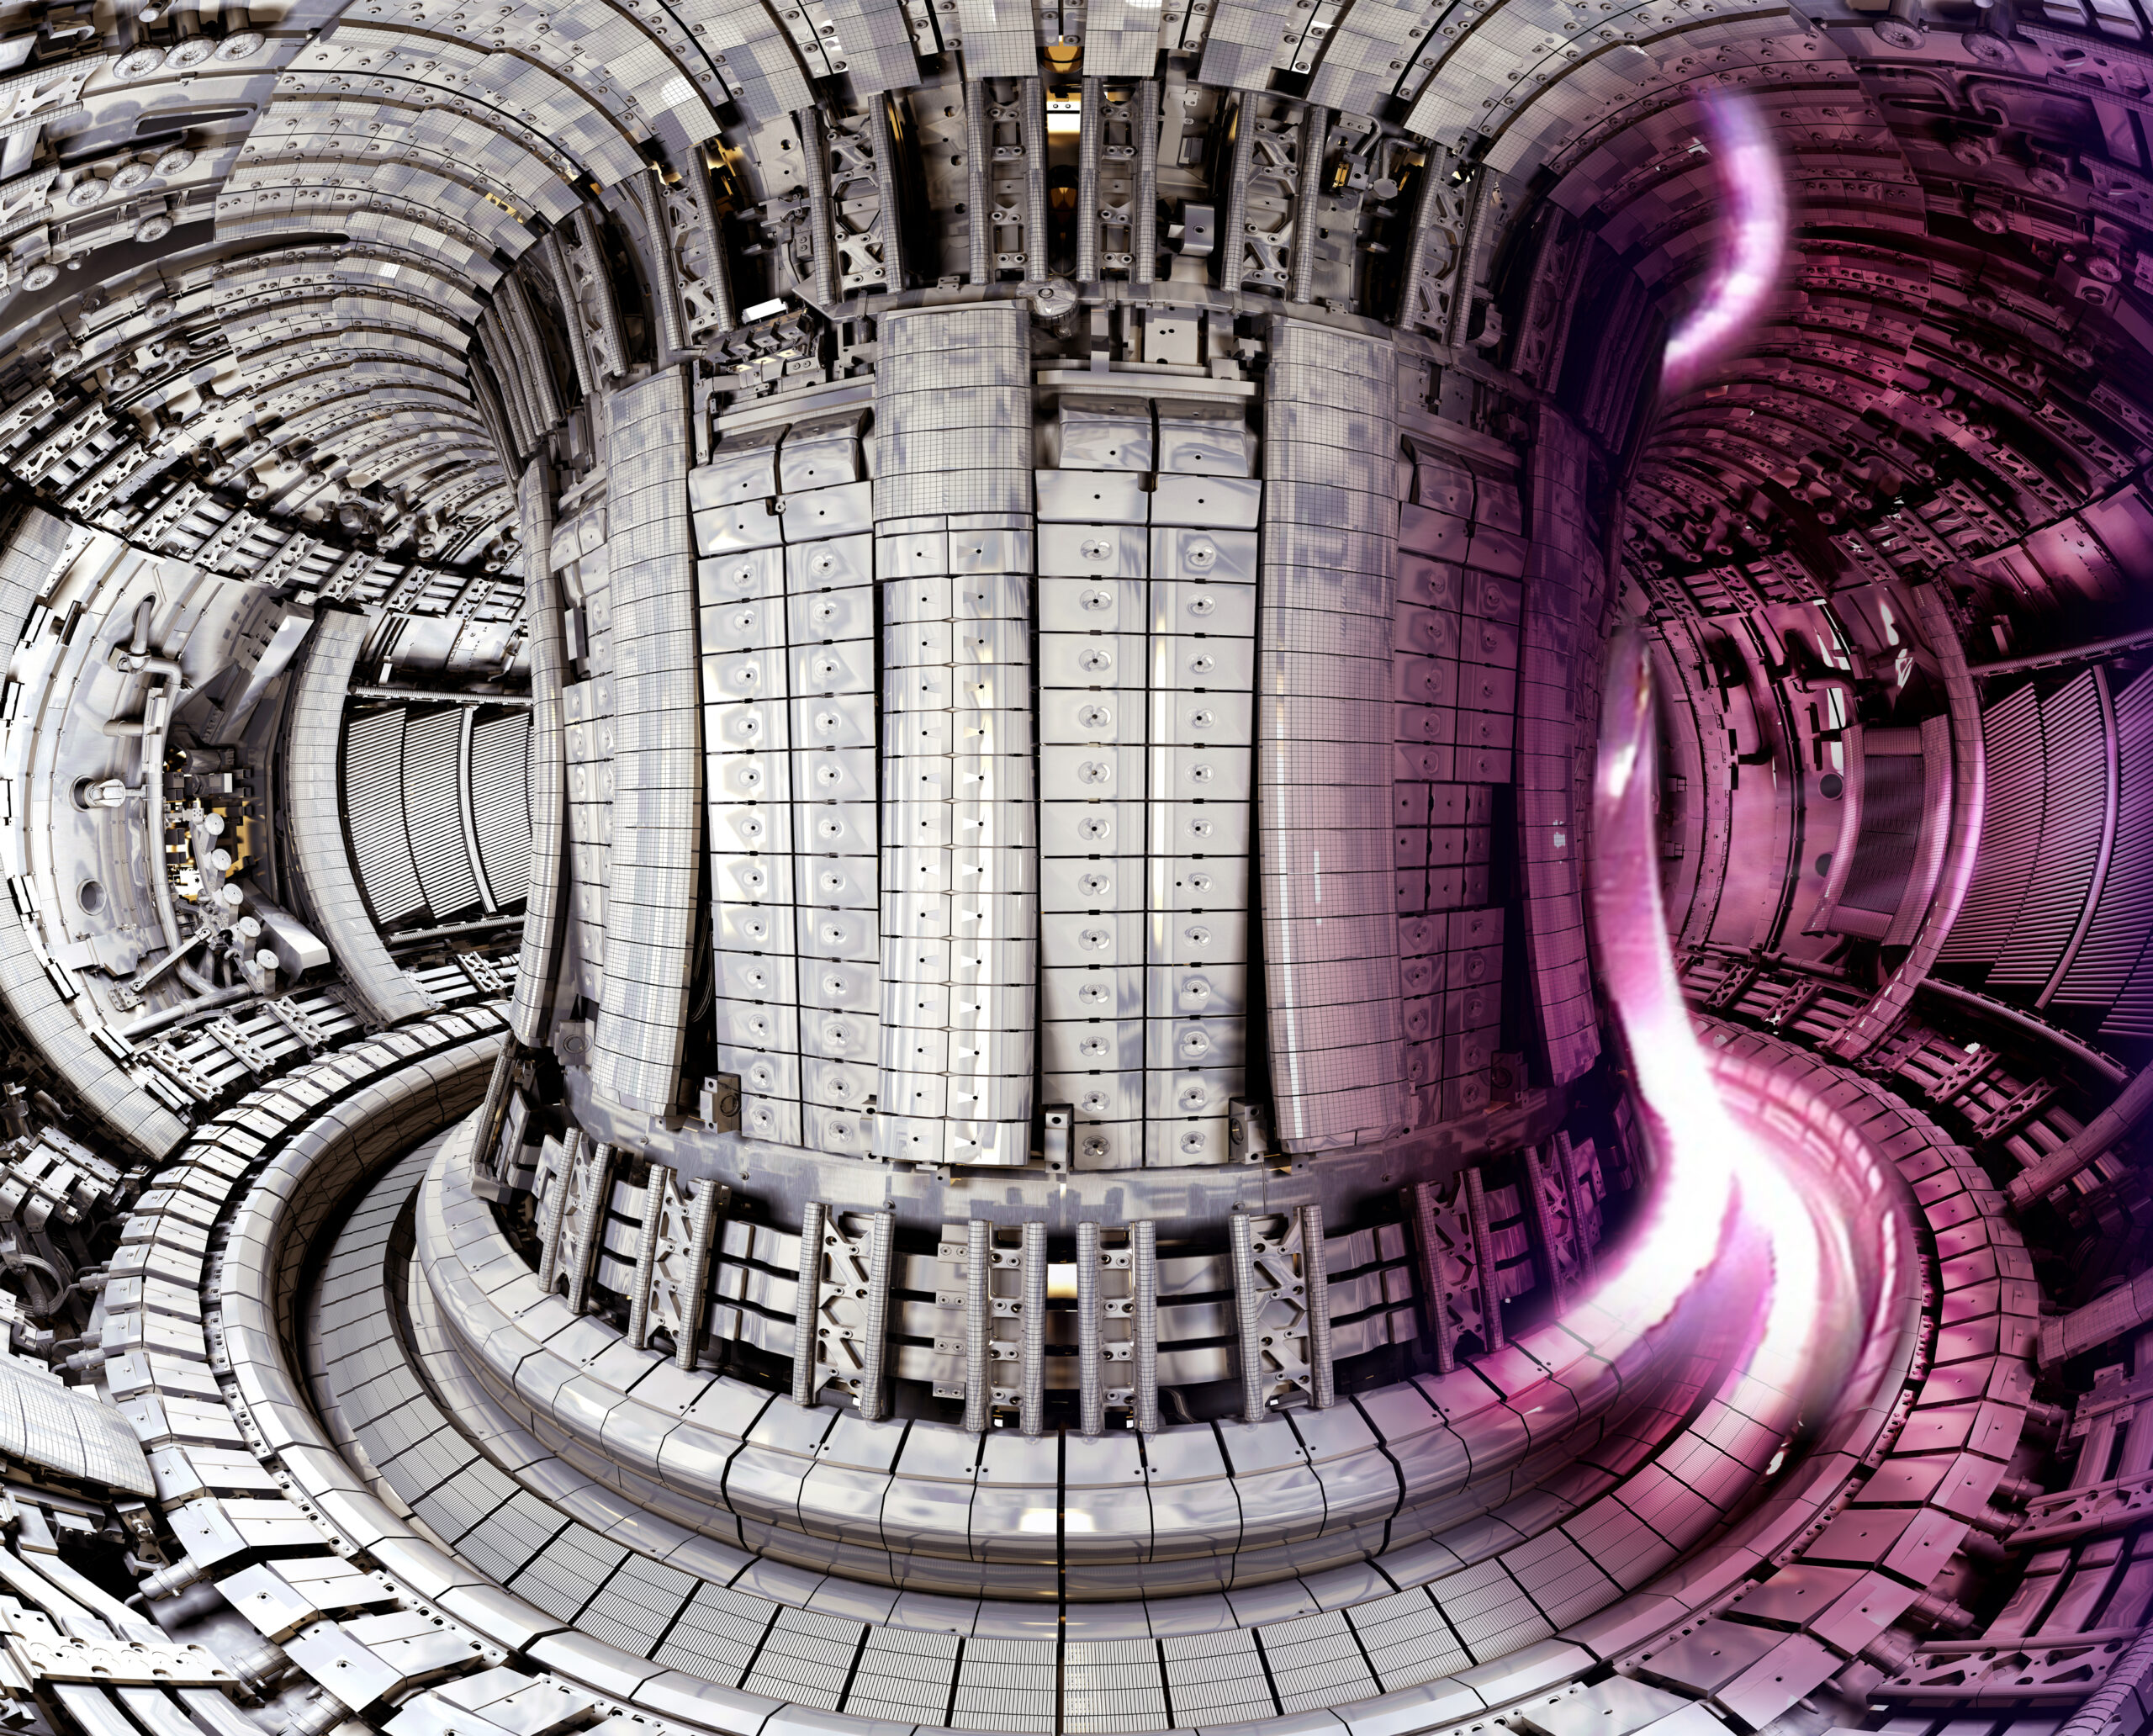
\includegraphics[width = 0.7\textwidth]{0 - introduction/images/JET.jpg}
        \caption{Illustration of the interior of the Joint European Torus (JET) reactor, located at the Culham Centre for Fusion Energy (CCFE). At the time of creation, JET was the largest tokamak in the world. (Source: CCFE)}
    \end{figure}

    \shortline

    The physical and numerical modeling of plasmas are crucial areas of study for tokamaks, as they aid in understanding and predicting the behavior of the hot plasma within the vessel. To achieve fusion, the plasma must be maintained at extremely high temperatures. Understanding its behavior is essential for optimizing the conditions in the tokamak and improving the fusion efficiency. Plasma modeling allows the simulation of various scenarios, such as changes in the magnetic fields or the heating methods used, and the observation of how these affect the plasma, allowing researchers and engineers to make informed decisions about how to increase the energy yield.

    In addition, plasma modeling helps to identify and resolve potential problems that may arise during the fusion reaction, such as instabilities in the plasma or unwanted interactions with the chamber walls. By using computer simulations, these issues can be identified and resolved before they occur outside the simulation, making the process safer and more efficient.
    
    \shortline

    \begin{remark}[Addendum]
        For a detailed introduction to plasmas and their modeling, and the great difficulties these pose in tokamak-like environments, I am currently working on a more detailed addendum, available at \cite{addendum}, currently a work in progress in parts. I have chosen to omit this in this document for brevity.
        
        This thesis shall make use only of the definitions and identities that follow, with all in a non-dimensionalized form.
    \end{remark}

    \shortline

    \begin{enumerate}
        \item  A positive deuterium ion and negative electric phase only, indexed via $\pm$ (or $*_{\pm}$), in (approximate) balance in particle density to give quasineutrality.
        
        Denoting the ratio of the mass of an electron to that of a deuterium ion as $\alpha$, we assume that $\alpha  \ll  1$.

        \item  The dimensionless constants, with approximate values under tokamak conditions calculated according to the JET operational values as given in \cite{Wes00}:
        \begin{itemize}
            \item  Cyclotron numbers, $\rmCy\!_{\pm}$:
            \begin{align}
                \rmCy\!_{+}  (=  - \alpha\rmCy\!_{-})  \approx    5.327\ldots\times 10^{2},  &&
                \rmCy\!_{-}                          \approx  - 1.957\ldots\times 10^{6}
            \end{align}
            
            \item  Light Mach number, $\rmM$:
            \begin{equation}
                \rmM  \approx  2.625\ldots\times 10^{- 3}
            \end{equation}
            
            \item  Plasma beta, $\beta$:
            \begin{equation}
                \beta  \approx  4.249\ldots 10^{- 3}
            \end{equation}

            \item  Interphase Knudsen numbers, $\rmKn_{\pm_{1}\pm_{2}}$, satisfying:
            \begin{itemize}
              \item  The dominant balance relations,
              \begin{equation}
                  \max\{\rmKn_{\pm\pm},  \rmKn_{\pm\mp}\}  =  |\rmCy\!_{\pm}|.
              \end{equation}
              
              \item  The consistency relation,
              \begin{equation}
                  \rmKn_{+-}  =  \alpha\rmKn_{-+}.
              \end{equation}
            \end{itemize}
            
            \item  Fluid Reynolds numbers, ${\rmRef}_{\pm_{1}\pm_{2}}$.
        \end{itemize}

        \item  The non-dimensionalized terms: 
        \begin{itemize}
            \item  Position and velocity vectors, $\bfx, \bfv  \in  \bbR^{3}$ respectively.
            
            \item  Time, $t  \in  \bbR$.
            
            \item  Electric and magnetic fields, $\bfE(\bfx; t), \bfB(\bfx; t)  \in  \bbR^{3}$ respectively.
            
            \item  Phase-specific particle distribution functions, $f_{\pm}(\bfx, \bfv; t)  \in  \bbR$.
            
            \item  Collision operators, $\bfC_{\pm_{1}\pm_{2}}[f_{\pm_{1}}, f_{\pm_{2}}](\bfx, \bfv; t)  \in  \bbR^{3}$, decomposing into dominant local and non-dominant non-local operators, $\bfC_{\pm_{1}\pm_{2}}^{(0)}[f_{\pm_{1}}|_{\bfx, \bfv; t}, f_{\pm_{2}}|_{\bfx, \bfv; t}](\bfx, \bfv; t),$ \\ $\bfdelta\bfC_{\pm_{1}\pm_{2}}[f_{\pm_{1}}, f_{\pm_{2}}](\bfx, \bfv; t)  \in  \bbR^{3}$ respectively, as
            \begin{equation}
                \bfC_{\pm_{1}\pm_{2}}  =  \bfC_{\pm_{1}\pm_{2}}^{(0)} + \frac{1}{\rmKn_{\pm_{1}\pm_{2}}{\rmRef}_{\pm_{1}\pm_{2}}}\bfdelta\bfC_{\pm_{1}\pm_{2}}.
            \end{equation}

            \item  Plasma mass and momentum density, $\rho_{\rmM}(\bfx; t)  \in  \bbR$ and $\bfp(\bfx; t)  \in  \bbR^{3}$ respectively, defined:
            \begin{align}
                \rho_{\rmM}  :=  \int_{\bfv}f_{+},  &&
                       \bfp  :=  \int_{\bfv}f_{+}\bfv.
            \end{align}

            \item  Plasma pressure, $p(\bfx; t)  \in  \bbR$, defined
            \begin{equation}
                p  :=  \frac{1}{3}\left(\int_{\bfv}f_{+}\|\bfv\|^{2} - \frac{1}{\rho_{\rmM}}\|\bfp\|^{2}\right).
            \end{equation}

            \item  Plasma charge and current density, $\rho_{\rmC}(\bfx; t)  \in  \bbR$ and $\bfj(\bfx; t)  \in  \bbR^{3}$ respectively, defined:
            \begin{align}
                \rho_{\rmC}  :=  \frac{\beta\rmCy\!_{+}}{2\rmM^{2}}\int_{\bfv}[f_{+} - f_{-}],  &&
                       \bfj  :=  \frac{\beta\rmCy\!_{+}}{2}\int_{\bfv}[f_{+} - f_{-}]\bfv.
            \end{align}

            \item  Plasma velocity and temperature, $\bfu(\bfx; t)  \in  \bbR^{3}$ and $\theta(\bfx; t)  \in  \bbR$ respectively, defined:
            \begin{align}
                  \bfu  :=  \frac{1}{\rho_{\rmM}}\bfp,  &&
                \theta  :=  \frac{1}{\rho_{\rmM}}p.
            \end{align}
        \end{itemize}

        \item  The (non-dimensionalized, convective timescale) equations:
        \begin{itemize}
            \item  The Boltzmann equations:
            \begin{equation}\label{eqn:Boltzmann equation}
                \partial_{t}f_{\pm} + \nabla_{\bfx}\cdot[f_{\pm}\bfv] + \rmCy\!_{\pm}\nabla_{\bfv}\cdot[f_{\pm}(\bfE + \bfv\wedge\bfB)]  =  \rmKn_{\pm\pm}\nabla_{\bfv}\cdot\bfC_{\pm\pm} + \rmKn_{\pm\mp}\nabla_{\bfv}\cdot\bfC_{\pm\mp}
            \end{equation}

            \item  The (local-in-space)leading-order Boltzmann equations:
            \begin{multline}\label{eqn:leading-order Boltzmann equation}
                \nabla_{\bfv}\cdot\left[\rmCy\!_{\pm}f_{\pm}(\bfE + \bfv\wedge\bfB) - \rmKn_{\pm\pm}\bfC_{\pm\pm}^{(0)} - \rmKn_{\pm\mp}\bfC_{\pm\mp}^{(0)}\right]  \\
                =  \frac{2}{\beta}\cdot\frac{1}{\rho_{\rmM}}\nabla_{\bfv}\cdot\left[f_{\pm}^{(0)}\left(\rmM^{2}\rho_{\rmC}\bfE + \bfj\wedge\bfB\right) - \nabla_{\bfv}\left[f_{\pm}^{(0)}\left(\bfj - \rmM^{2}\rho_{\rmC}\bfu\right)\cdot\left(\bfE + \bfu\wedge\bfB\right)\right]\right]  \\
                + \calO\left[1, \frac{1}{\rmRef}\right],
            \end{multline}

            \item  The (leading-order) magnetohydrodynamic (MHD) equations, under the assumption of exact thermalization:
            \begin{align}
                \partial_{t}\rho_{\rmM} + \nabla_{\bfx}\cdot\bfp  &=  0  \label{eqn:mass conservation}  \\
                \rmM^{2}\partial_{t}\rho_{\rmC} + \nabla_{\bfx}\cdot\bfj  &=  0,
            \end{align}
            \vspace{-25pt}
            \begin{multline}
                \partial_{t}\bfp + \left(\nabla_{\bfx}\cdot\left[\rho_{\rmM}\bfu^{\otimes 2}\right] + \nabla_{\bfx}p\right) - \frac{2}{\beta}\left(\rmM^{2}\rho_{\rmC}\bfE + \bfj\wedge\bfB\right)  \\
                =  - \int_{\bfv}\left[\frac{1}{{\rmRef}_{++}}\bfdelta\bfC_{++} + \cdots + \frac{1}{{\rmRef}_{--}}\bfdelta\bfC_{--}\right]
            \end{multline}
            \vspace{-15pt}
            \begin{multline}
                \frac{3}{2}\partial_{t}p + \left(\frac{3}{2}\nabla_{\bfx}\cdot[p\bfu] + p\nabla_{\bfx}\cdot\bfu\right) - \frac{2}{\beta}\left(\bfj - \rmM^{2}\rho_{\rmC}\bfu\right)\cdot(\bfE + \bfu\wedge\bfB)  \\
                =  - \int_{\bfv}\left[\frac{1}{{\rmRef}_{++}}\bfdelta\bfC_{++} + \cdots + \frac{1}{{\rmRef}_{--}}\bfdelta\bfC_{--}\right]\cdot(\bfv - \bfu)  \label{eqn:energy conservation}
            \end{multline}

            \item  Maxwell's equations:
            \begin{align}
                \rmM^{2}\partial_{t}\bfE  &=  \nabla_{\bfx}\wedge\bfB - \bfj,  &
                        \partial_{t}\bfB  &=  - \nabla_{\bfx}\wedge\bfE,  \label{eqn:Maxwell's equations transient}  \\
                  \nabla_{\bfx}\cdot\bfE  &=  \rho_{\rmC},  &
                  \nabla_{\bfx}\cdot\bfB  &=  0.  \label{eqn:Maxwell's equations steady-state}
            \end{align}
        \end{itemize}
    \end{enumerate}

    We also make use of the following lemma:

    \begin{lemma}[Phase-restricted momentum and energy conservation on $(\bfC_{\pm_{1}\pm_{2}}^{(0)})_{\pm_{1}\pm_{2}}$]\label{lem:phase-restricted conservation on local collision operators}
        The following identities on $(\bfC_{\pm_{1}\pm_{2}}^{(0)})_{\pm_{1}\pm_{2}}$ hold:
        \begin{itemize}
            \item  The following two identities hold on $\bfC_{\pm\pm}^{(0)}$:
            \begin{align}
                \int_{\bfv}\bfC_{\pm\pm}^{(0)}           =  \calO[\epsilon_{\pm\pm}],  &&
                \int_{\bfv}\bfC_{\pm\pm}^{(0)}\cdot\bfv  =  \calO[\epsilon_{\pm\pm}],
            \end{align}
            where
            \begin{equation}
                \epsilon_{\pm\pm}  :=  \frac{1}{\rmKn_{\pm\pm}{\rmRef}_{\pm\pm}}.
            \end{equation}
            \item  The following two identities hold on $\bfC_{+-}^{(0)}$ and $\bfC_{-+}^{(0)}$:
            \begin{align}
                \int_{\bfv}\left[\bfC_{+-}^{(0)} + \bfC_{-+}^{(0)}\right]           =  \calO[\epsilon_{+-}],  &&
                \int_{\bfv}\left[\bfC_{+-}^{(0)} + \bfC_{-+}^{(0)}\right]\cdot\bfv  =  \calO[\epsilon_{+-}],
            \end{align}
            where
            \begin{equation}
                \epsilon_{+-}  :=  \frac{1}{\rmKn_{+-}}\max\left\{\frac{1}{{\rmRef}_{++}}, \frac{1}{{\rmRef}_{+-}}, \frac{\alpha}{{\rmRef}_{--}}, \frac{\alpha}{{\rmRef}_{-+}}\right\}.
            \end{equation}
        \end{itemize}
    \end{lemma}
